%!TEX root = ../Main.tex
\begin{wrapfigure}[13]{r}{.45\textwidth}
	\vspace{-2em}
	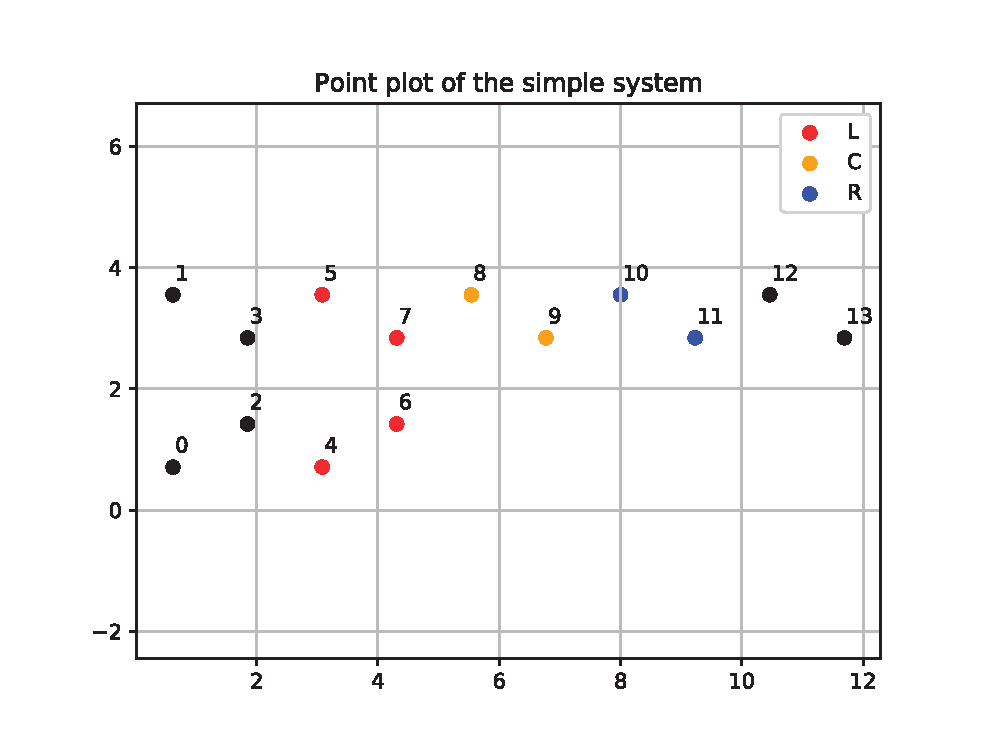
\includegraphics[width=.45\textwidth]{Figures/pointplot.eps}
	\caption{Figure showing the simple system. The atoms 4-11 is the device itself while the black atoms are the semi-infinite chain of atoms around the device.}\label{inlinepointplot}
\end{wrapfigure}
In the following sections, the focus will be to present and explain how to calculate band structures, local density of states and transmission through Python-programming, using the tight-binding approximation for any periodic structure. For simplicity, all initial examples and calculations will be done on a simple system, to make sure the different steps are easy to follow. The system can be seen in \cref{inlinepointplot}. Note how the atoms have indices according to their position. The device consist of a left (red) contact, a right (blue) contact and the atoms in between (yellow). Around the device one finds the semi-infinite chain of atoms.
\subsection{Creating the on-site Hamiltonian and hopping matrices}
The first and most essential parts needed for calculations is the \textit{on-site} Hamiltonian \(\mathbf{h_0}\) and the \textit{hopping} matrices \(\mathbf{V},\ \mathbf{V}^{\dagger}\). The starting point is a matrix, containing a set of coordinates \(x_0,y_0,z_0\), representing atom positions and a set of unit vectors \(\mathbf{u}_x, \ \mathbf{u}_y, \ \mathbf{u}_z\). The unit vectors will be the basis of the unit cell containing all atom coordinates. From now on, only the x and y coordinates will be considered as graphene is considered purely a 2D material.
% \begin{figure}[h]
% 	\centering
% 	\begin{subfigure}[b]{0.45\textwidth}
% 		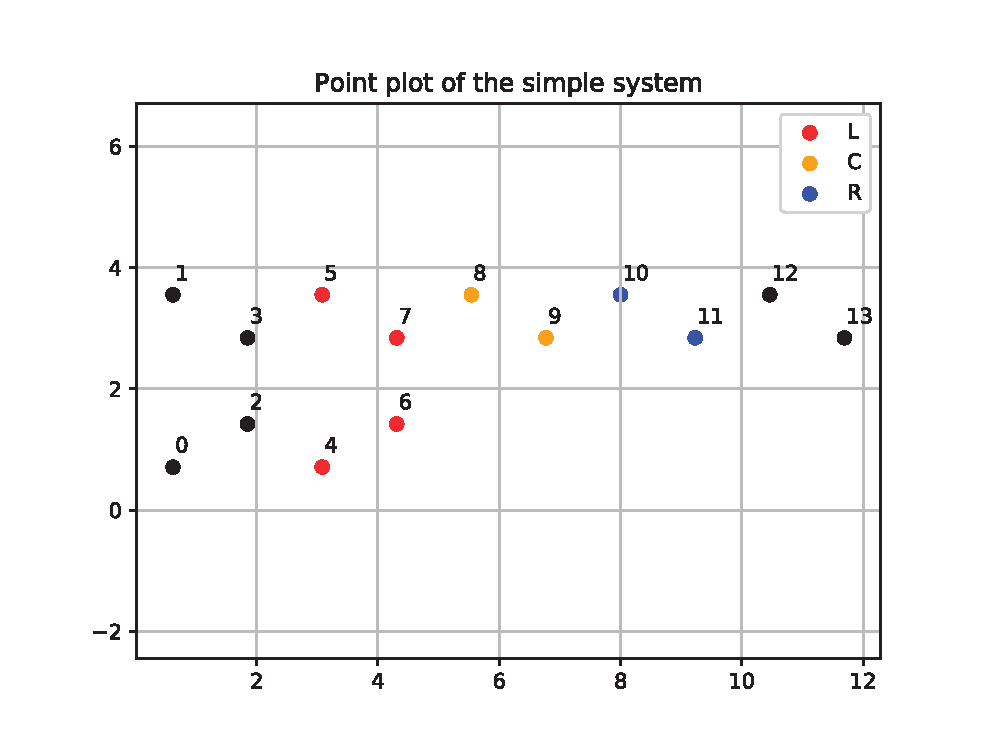
\includegraphics[width=\textwidth]{Figures/pointplot.eps}
% 		\caption{Figure showing the simple system. Every atom in the unit cell has an index, here from 4 to 11. The blue and red colours mark the left and right contacts of the system. The black parts represent the rest of reduced semi-infinite chain.}
% 		\label{pointplot}
% 	\end{subfigure}
% 	~ %add desired spacing between images, e. g. ~, \quad, \qquad, \hfill etc.
% 	%(or a blank line to force the subfigure onto a new line)
% 	\begin{subfigure}[b]{0.45\textwidth}
% 		\includegraphics[width=0.7\textwidth]{Figures/BetaBandstructures.eps}
% 		\caption{Figure showing the band structure of the simple system.}
% 		\label{bandssimple}
% 	\end{subfigure}
% 	\vskip\baselineskip %add desired spacing between images, e. g. ~, \quad, \qquad, \hfill etc.
% 	%(or a blank line to force the subfigure onto a new line)
% 	\begin{subfigure}[t]{0.45\textwidth}
% 		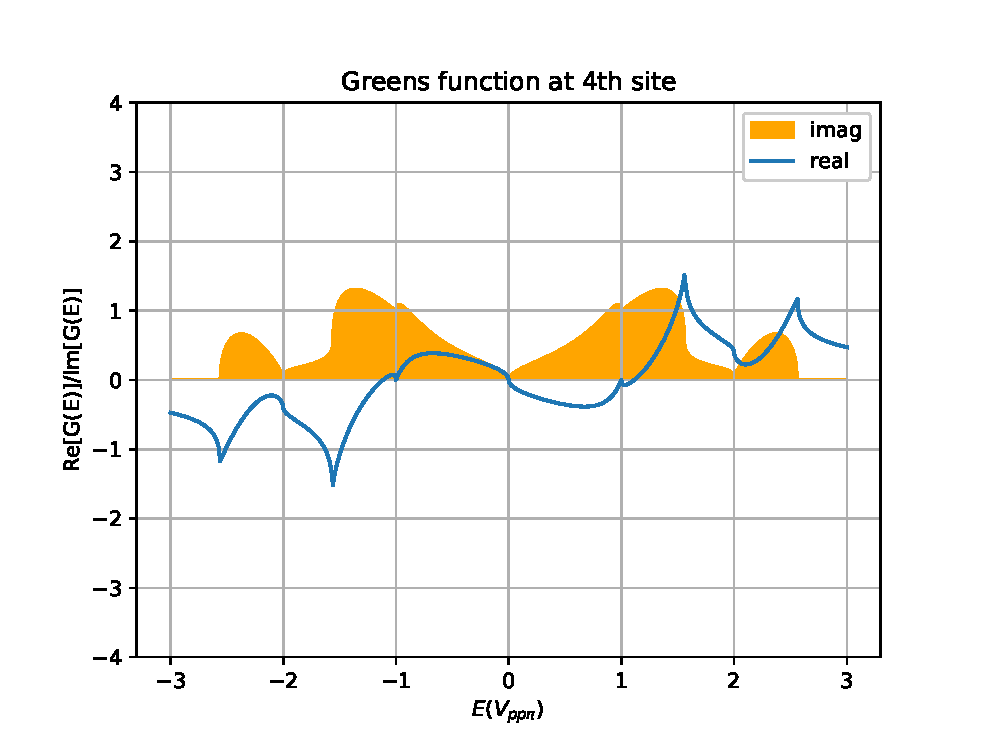
\includegraphics[width=\textwidth]{Figures/BetaimrealTE.eps}
% 		\caption{A plot showing the real and imaginary part of Green's function at the zeroth site resulting from the recursion routine on the simple system. Note that the yellow imaginary part is the representation of the local density of states.}
% 		\label{LDOSsimple}
% 	\end{subfigure}
% 	~
% 	\begin{subfigure}[t]{0.45\textwidth}
% 		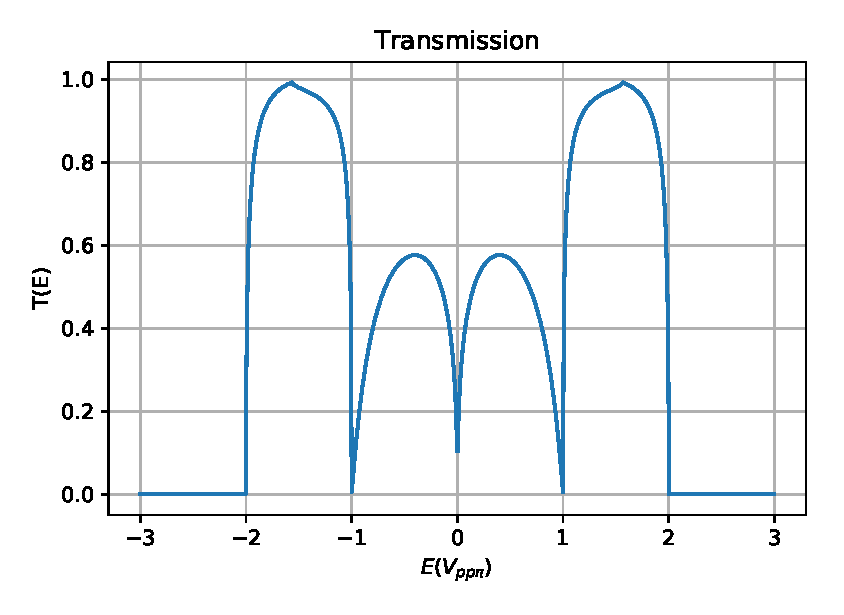
\includegraphics[width=\textwidth]{Figures/BetaTE.eps}
% 		\caption{Figure showing the resulting transmission through the simple system}
% 		\label{Transsimple}
% 	\end{subfigure}
% 	\caption{Figure of the different calculations executed on the simple system, using the developed scripts. }\label{eksamplefigure}
% \end{figure}
The on-site Hamiltonian represents the interaction of atoms within the unit cell and the hopping matrices represents the interaction of atoms between periodically repeated unit cells.
\begin{figure}[ht]
 \centering
 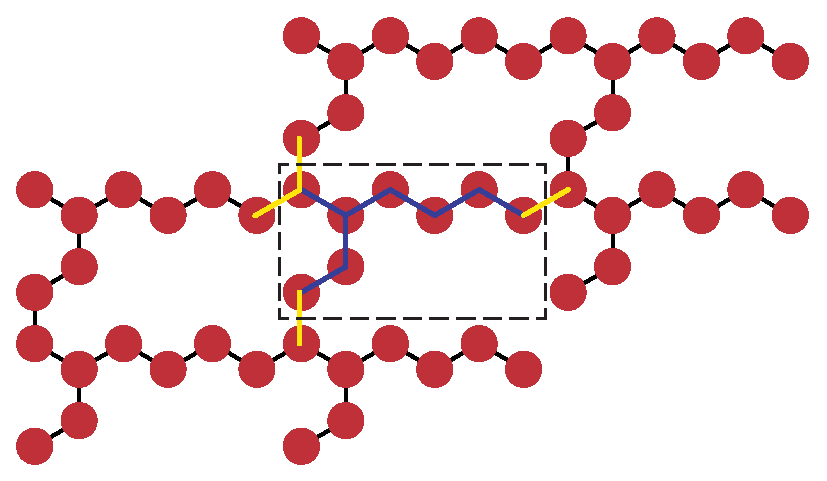
\includegraphics[width=.7\textwidth]{Figures/atomreffig.eps}
 \caption{Visual representation of the periodic simple system. The atoms surrounded by the black box in the centre represents the unit cell. The neighbouring boxes are unit cells repeated periodically once in every direction. Blue connections are onsite hops. Yellow are offsite hops.}
 \label{atomrepfig}
\end{figure}
In \cref{atomrepfig} a visual representation of the simple systems with periodically repeated unit cells can be seen. For the rest of the report, the on-site Hamiltonian will all ways be the centre cell while the hopping matrices will be the cells surrounding the on-site Hamiltonian (See \cref{repfig} for a generalised visual representation of the concept).\newline
In order to find these hop we start off with a set of coordinates for the unit cell atoms as well with the lattice unit vectors. In order to get the onsite hop matrix we use what is called the vector outer product. This means that every coordinate set is compared to every other coordinate set. In our case, we want to find the nearest neighbours. Every two atoms within a distance of \SI{1.6}{\angstrom} is considered nearest neighbours. A function called \textit{Onsite} have been developed to do just this. In \cref{npouter} the function can be seen.
\im{Listings/Functions.py}{33}{38}
\vspace{-1\baselineskip}
\captionof{listing}{The outer operator in numpy is manifested as two nested loops. On lines 34-36 each atomic distance is calculated. Line 37 replaces all nearest neighbour distances with an input potential, leaving the rest as zero. Lastly the diagonal is subtracted from the matrix on line 38.\label{npouter}}\vspace{\baselineskip}
The function produces a matrix which contain all distances between all atoms in the unit cell. The tight-binding model dictates that only atoms with a specific inter-atomic distance interact. Therefore the function has implemented a threshold (\cref{npouter} line 37) to determine whether a given distance is too great for interaction or small enough for interaction. All distances above the threshold will be changed to a 0-element in the on-site Hamiltonian matrix, representing zero interaction and all distances below the threshold will be changed to 1 to represent interaction between atoms. Finally The on-site Hamiltonian is multiplied with a on-site potential (scalar). The on-site potential \(V_{pp\pi}\) differs depending on the system. Lastly the diagonal is subtracted as these elements represent the electrons average energy on each site. Remember that \(\epsilon_0 = 0\). Now the on-site Hamiltonian is complete and the product is a matrix containing 0's and 1's to represent interaction between atoms in a unit cell. \newline
Moving on to the hopping matrices one first has to realise that the interactions are happening in a 2D plane. This has to be kept in mind when describing interaction between unit cells repeated in all directions in the plane. Effectively this means that six hopping matrices should be created. One in the x-direction, one in the y-direction, one in the xy-direction and their hermitian conjugates. Graphically this corresponds to a structure of this kind:
\begin{figure}[H]
	\centering
	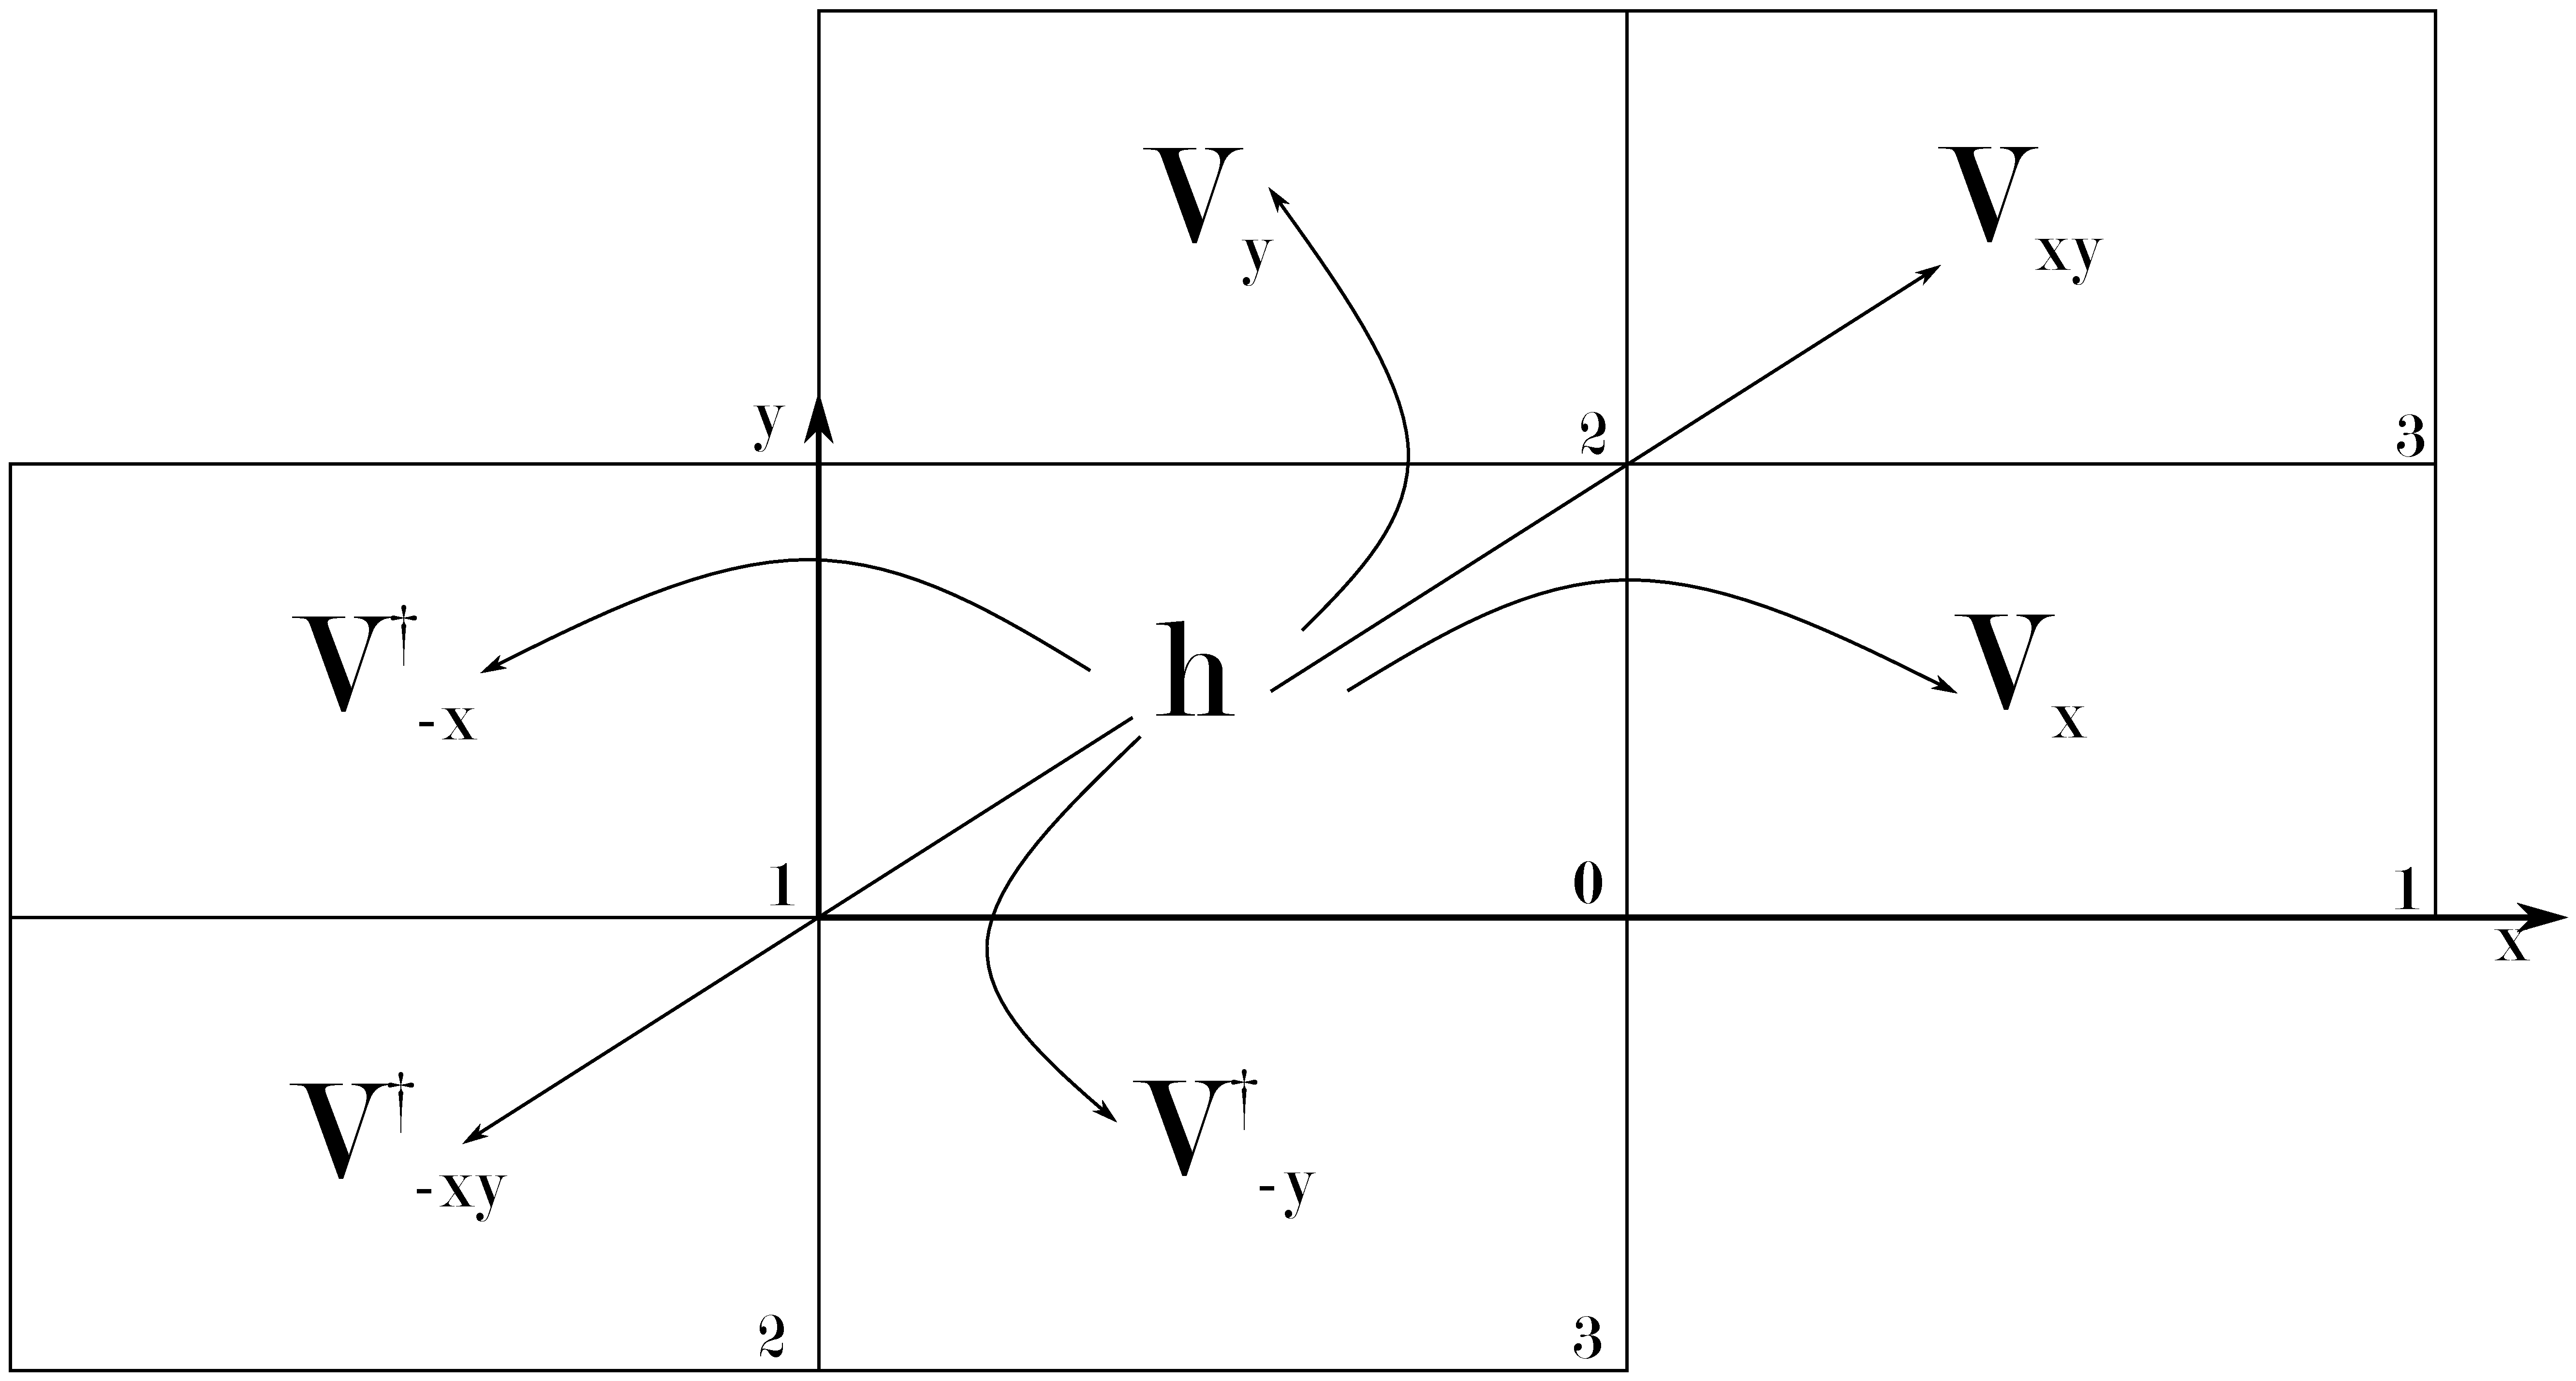
\includegraphics[width = 0.7\textwidth]{Figures/repfig.eps}
	\caption{Representative figure of how the on-site Hamiltonian along with its hopping matrices are structured}
	\label{repfig}
\end{figure}
In practice this is done by shifting the original \(x_0,y_0\) coordinates by the given unit vectors \(\mathbf{u}_x,\mathbf{u}_y\). By addition of the unit vectors to the original coordinate matrix one can get three new coordinate matrices \(\mathbf{xy}_{shift-x}=x_0,y_0 + \mathbf{u}_x\), \(\mathbf{xy}_{shift-y}=x_0,y_0 + \mathbf{u}_y\) and \(\mathbf{xy}_{shift-xy}=x_0,y_0 + \mathbf{u}_x+\mathbf{u}_y\). With these three matrices what follows is basically the same method used to get the on-site Hamiltonian. The only difference being that it will be distances between atoms in the on-site Hamiltonian and the shifted matrices respectively. That way it is the distance, and thus the interaction, between the on-site Hamiltonian and the repeated unit cells that is calculated. The three resulting hopping matrices are denoted \(\vb{V}_{x}\), \(\vb{V}_{y}\) and \(\vb{V}_{xy}\). They represent interaction (hopping) in the "forward" direction (left-to-right) (See \cref{repfig}). To create the hopping matrices hopping in the "backwards" (right-to-left) direction (See \cref{repfig}) one simply has to transpose the hopping matrices. These matrices are denoted with a dagger: \(\vb{V}_{x}^{\dagger}\), \(\vb{V}_{y}^{\dagger}\) and \(\vb{V}_{xy}^{\dagger}\). To get an idea of how such matrices looks like, see \cref{matrixmap}, where the resulting matrix-maps from a small 12-atom graphene unit cell are shown. It has been stitched together like in \cref{repfig}.
\begin{figure}[ht]
	\centering
	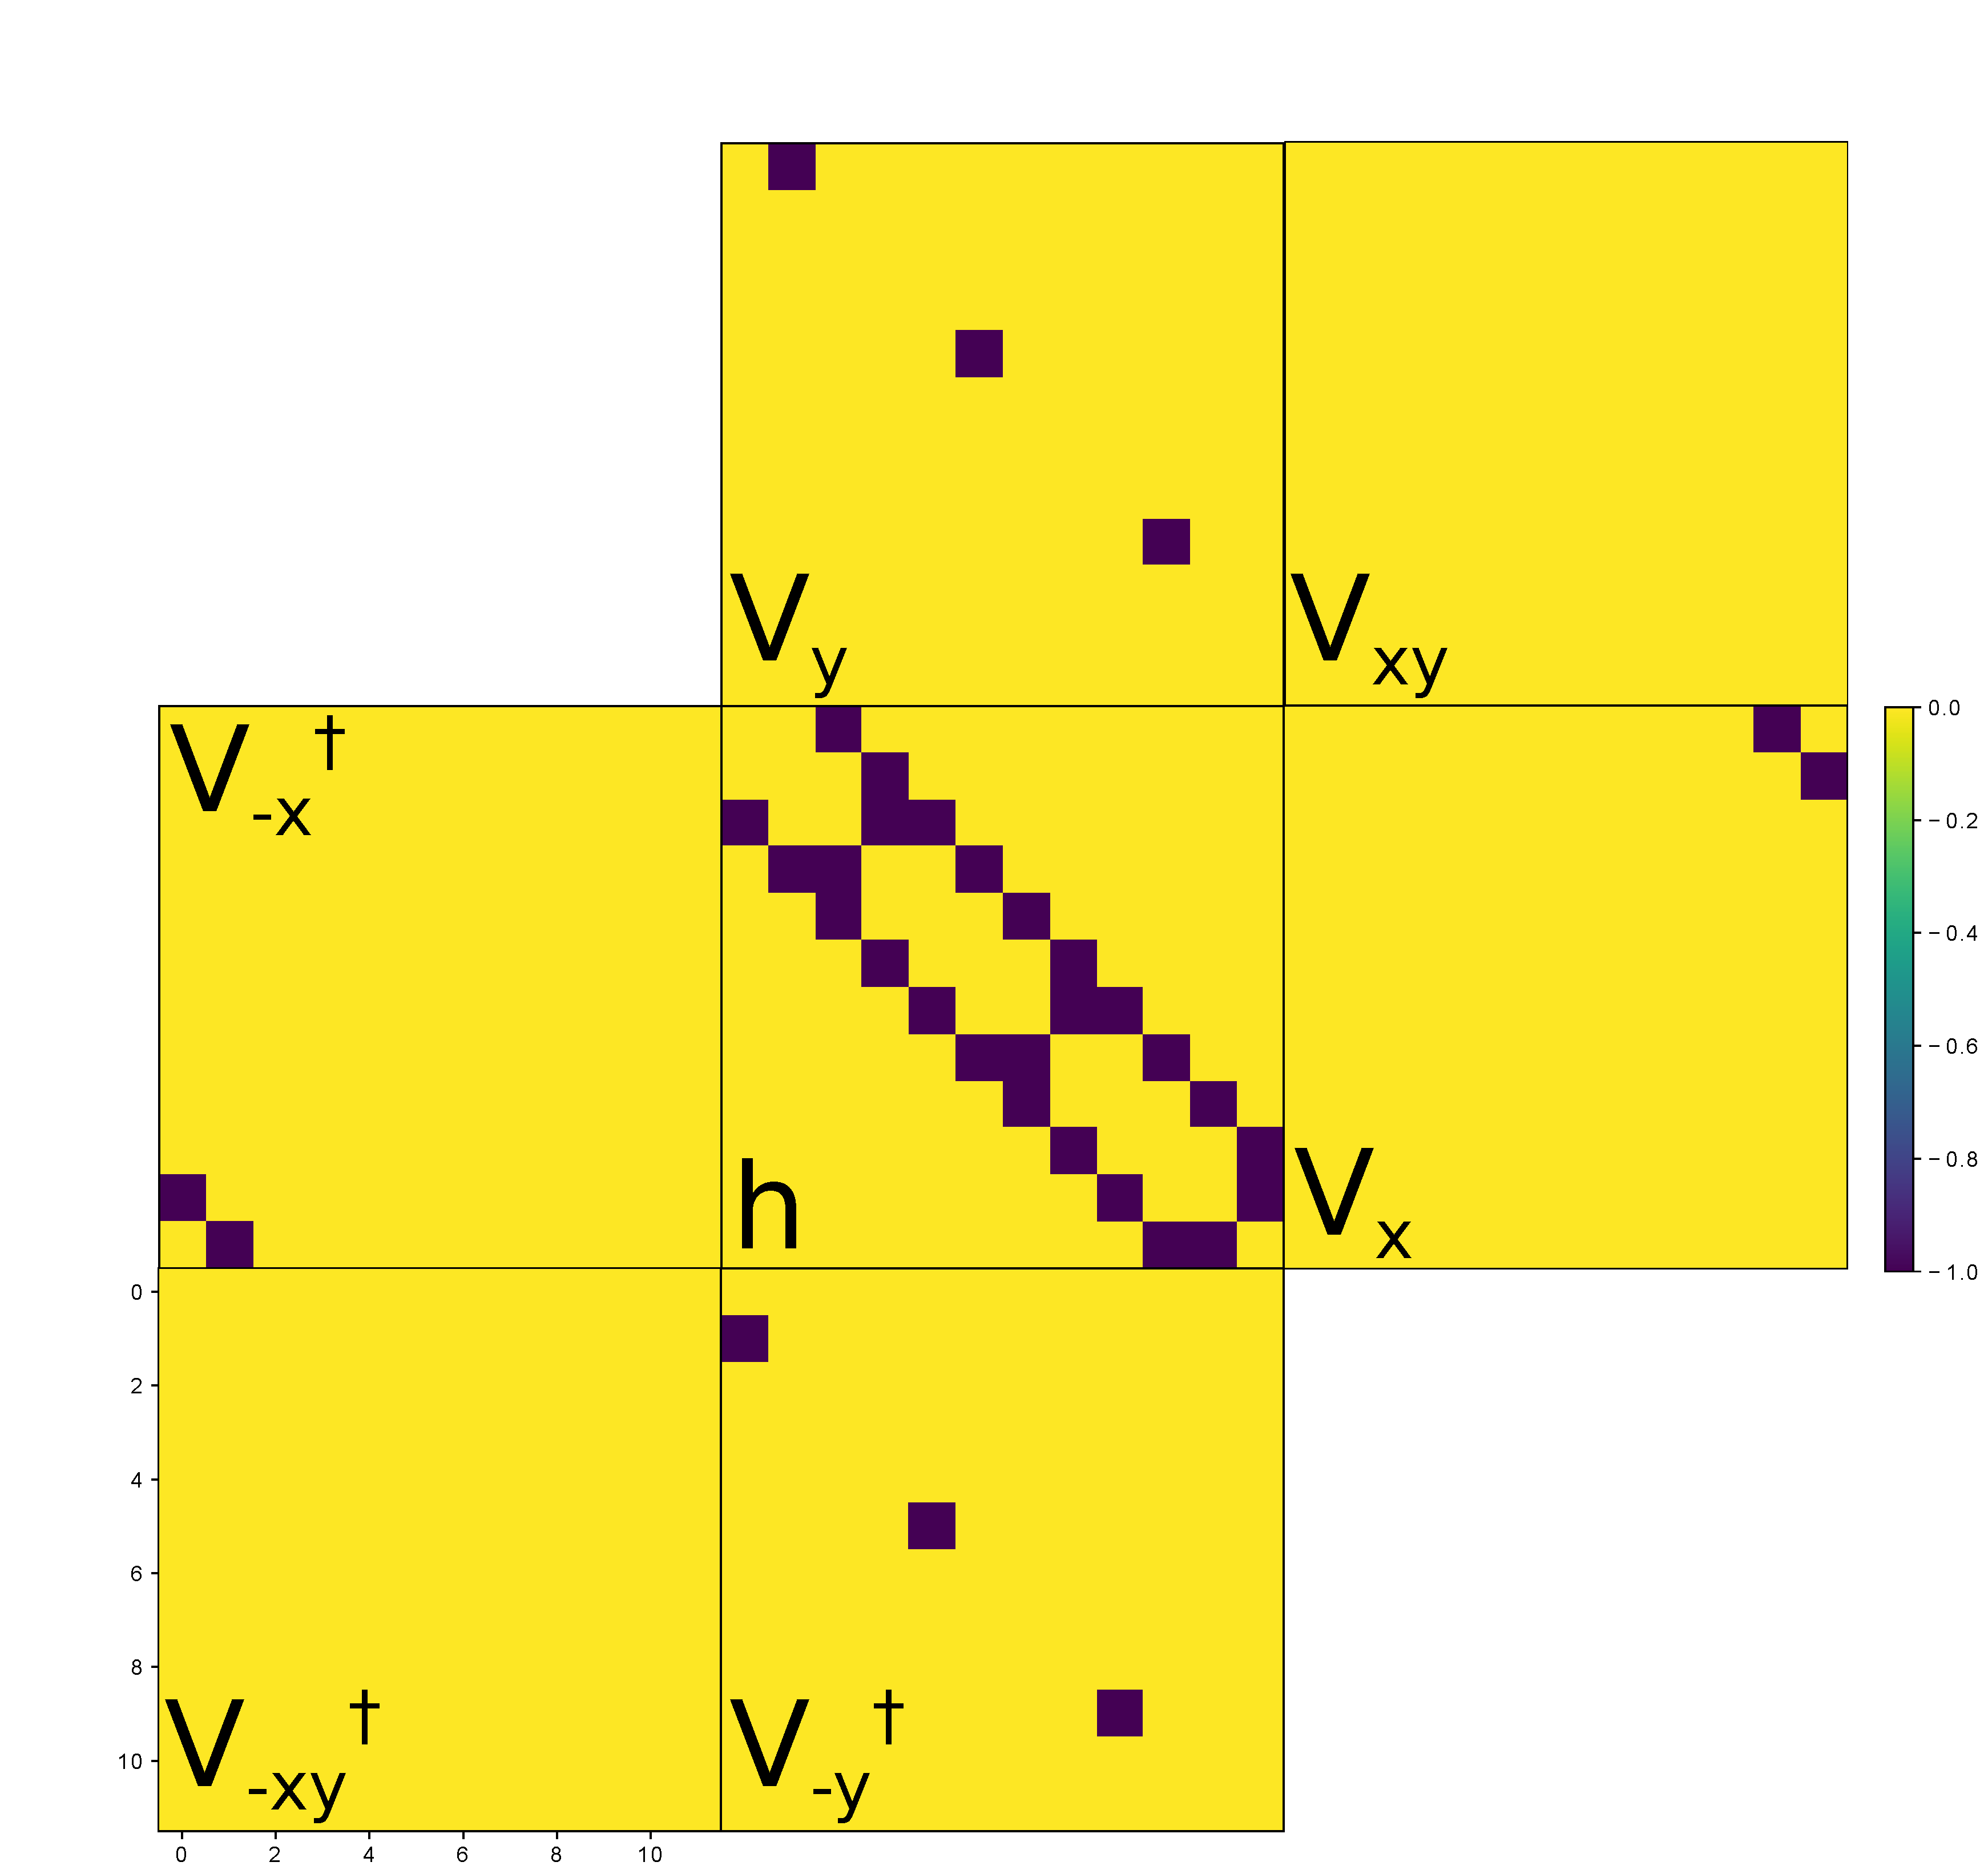
\includegraphics[width=0.7\textwidth]{Figures/stitch.eps}
	\caption{Matrix maps from calculation on an arbitrary graphene system with a unit cell of 12 atoms. The on-site Hamiltonian along with all its hopping matrices are stitched together like in figure \cref{repfig}. All the dark spots represent a hopping of an electron to its nearest neighbour i.e. a 1 element and yellow represents a 0 element}
	\label{matrixmap}
\end{figure}
\subsection{Defining the full Hamiltonian and solving the Schr\"{o}dinger equation}\label{FullHam}
Now that the on-site Hamiltonian along with its hopping matrices have been created, the next step is to create the full Hamiltonian in order to solve the Schr\"{o}dinger equation for the system as a whole. This is an eigen-value/vector problem. The Schr\"{o}dinger equation needs to be solved to get the eigen energies for the system as they will be used to produce band structure plots later on. In essence the full Hamiltonian denoted \(\vb{H}\) is a sum of the on-site Hamiltonian and its corresponding hopping matrices multiplied by a complex exponential function that has the appropriate phase relative to the hopping matrix. Remember that the electrons moves as waves in the periodic system. Because of the periodicity it is practical to use the reciprocal space. Here the electron can move from \textit{k}-point to \textit{k}-point, where \(k\) represents a continuous variable between 0 and \(\pi\) along the \(\dfrac{1}{x}\)- and \(\dfrac{1}{y}\)-axis (hence the term ``reciprocal space'').
This means that when moving from one  \textit{k}-point to another, one needs to multiply the appropriate parts with a Bloch phase:
\begin{align}\label{hamileq}
	\vb{H}(k_x,k_y) = \vb{h}_0 & + (\vb{V}_{x}e^{-ik_x} + \vb{V}_{x}^{\dagger}e^{ik_x}                   \nonumber   \\
	                           & + \vb{V}_{y}e^{-ik_y} + \vb{V}_{y}^{\dagger}e^{ik_y}                               \\
	                           & + \vb{V}_{xy}e^{-ik_x}e^{-ik_y} + \vb{V}_{xy}^{\dagger}e^{ik_x}e^{ik_y}) \nonumber
\end{align}
Using the full Hamiltonian, the Schrodinger equation can be solved
\begin{align}
	\vb{H}(k_x,k_y)\vb*{\phi}_{k} = \vb*{\epsilon}_n (k_x,k_y) \vb*{\phi}_k
\end{align}
Where \(\vb*{\phi}_k\) is the electron wavefunctions and \(\vb*{\epsilon}(k_x,k_y)\) is the eigenenergies. \\
In practice this is done by defining a function, here called \textit{Hkay}, that takes the on-site Hamiltonian, the hopping matrices, and \(k_{x/y}\) as inputs and outputs the eigenvalues, using numpy's \textit{numpy.linalg.eigh}, which diagonalises the Hamiltonian matrix. The number of eigenvalues in the output corresponds to the dimension of the full Hamiltonian. In \cref{fullhamil} the code for the function is shown.
\im{Listings/Functions.py}{73}{80}
\vspace{-1\baselineskip}
\captionof{listing}{Function producing the full hamiltonian, corresponding to \cref{hamileq} the inputs x and y corresponds to the \(k_x\),\(k_y\) .\label{fullhamil}}\vspace{\baselineskip}
\subsection{Producing band structures}
\begin{wrapfigure}[20]{r}{.30\textwidth}
	\vspace{-2em}
	\includegraphics[width=0.30\textwidth]{Figures/BetaBandstructures.eps}
	\caption{Figure showing the band structure of the simple system.}\label{bandssimple}
\end{wrapfigure}
%An important intrinsic information in any solid state matter is of course the band structure as it gives information about allowed electron energies at different points in the material. Specifically for NPG, the band structure may be used to track the changes of electronic transport upon changing the bridges connecting GNR's within NPG.
In order to calculate and visualise the band structure of the simple system, one need to define the full Hamiltonian \(\vb{H}\) in two directions. When working with band structures and periodic systems it is common to note points in space with respect to the \textit{Brillouin Zone} which is a primitive cell in reciprocal space. Therefor
a continuous variable \(k\) is introduced. it extends in two directions in (\(-k_{x}\)) and (\(k_{y}\)), which correspond to lengths between the symmetry points \(X\), \(\Gamma\) and \(Y\) in the Brillouin zone. Here \(\Gamma\) is the origin \((0,0)\). Practically this corresponds to making two plots, one for each pair of symmetry points. The y-values in each plot correspond to the eigenvalues obtained by the \textit{Hkay} function described in \cref{FullHam}. The number of eigen energies, and effectively the number of bands in the plot is dictated by the dimensions of the Hamiltonian, which again is dictated by the number of unit cell atoms. \textit{n}-atoms \(\rightarrow\) \(n\times n\)-matrix \(\rightarrow\) \textit{n} eigenenergies (bands). However plots produced in this report will only show a few of these bands in a small energy range. In the case of the simple system, the full Hamiltonian for obtaining the eigen energies that corresponds to directions \(X\) and \(Y\) are:\begin{align}
	X: \ \vb{H}_{X} = \vb{h}_0 + (\vb{V}_{x}e^{ik_x} + \vb{V}_{x}^{\dagger}e^{-ik_x} + \vb{V}_{y} + \vb{V}_{y}^{\dagger} + \vb{V}_{xy}e^{ik_x} + \vb{V}_{xy}^{\dagger}e^{-ik_x}) \\
	Y: \ \vb{H}_{Y} = \vb{h}_0 + (\vb{V}_{x} + \vb{V}_{x}^{\dagger} + \vb{V}_{y}e^{-ik_y} + \vb{V}_{y}^{\dagger}e^{ik_y} + \vb{V}_{xy}e^{-ik_y} + \vb{V}_{xy}^{\dagger}e^{ik_y})
\end{align}Using the eigenvalues as y-values in the two plots, putting the two plots together will yield a final plot of the band structure shown in \cref{bandssimple}.
